\RequirePackage{silence}
\WarningFilter{latex}{Writing or overwriting file}

\begin{filecontents*}[overwrite]{\jobname.xmpdata}
\Title{Modelli architetturali per lo sviluppo software: l'approccio basato sui microservizi}
\Author{Lorenzo Paolo Cocchinone}
\Language{it-IT}
\Subject{Sviluppo di un applicativo basato sull'approccio a microservizi}
\Keywords{Microservizi\sep Springboot\sep Docker\sep Kubernetes\sep Maven}
\end{filecontents*}

\documentclass[a4paper,oneside,11pt,openright,table]{book}

\usepackage{packages}

\begin{document}

\frontmatter
\begin{titlepage}
\changepage{}{}{}{-7.5 mm}{}{}{}{}{}
% parametri per cambiare le dimensioni di una singola pagina in ordine:
% {textheight}{textwidth}{evensidemargin}{oddsidemargin}{columnsep}
% {topmargin}{headheight}{headsep}{footskip}
% se voglio centrare la pagina devo mettere bindingoffset/2
% i primi 5 parametri posso usarli con \changetext


\begin{center}

\includegraphics[width=.15\columnwidth, angle=0]{capitoli/immagini/fronte/logo-unisa.pdf}\\ % height
\vspace{0.5cm}
{\Large \scshape Università degli Studi di Salerno}\\
\vspace{0.5cm}
{\Large Dipartimento di Informatica}\\
\vspace{0.5cm}
{\Large Corso di Laurea Triennale in Informatica}\\
\vspace{1.5cm}
{\Large \scshape Tesi di Laurea} \\
\vspace{3cm}
{\Huge \bfseries MODELLI ARCHITETTURALI PER LO SVILUPPO SOFTWARE: L'APPROCCIO BASATO SUI MICROSERVIZI} \\
\vspace{3cm}

\begin{minipage}[t]{7cm}
\flushleft
{\large \textsc{Relatore}}

{\large Prof. Rita Francese} \\
{\large $ $} \\
Università degli Studi di Salerno \\[0.25cm]
\end{minipage}
\hfill
\begin{minipage}[t]{7cm}
\flushright
{\large \textsc{Candidato}}

{\large \textbf{Lorenzo Paolo Cocchinone}} \\
Matricola: 0512105326
\end{minipage}

\vspace{2.5cm}

{\small Anno Accademico 2021-2022} %\\
%
%
\end{center}

\end{titlepage}

\begin{titlepage}
\nonumber
\null \vspace {\stretch{1}}
\begin{flushright}

\textit{Try again, I'm wishin' you well! \\
But you will never roast me better than I roast myself \\
Mori Calliope.}

\end{flushright}
\end{titlepage}

\pagenumbering{roman}
\chapter*{Abstract}
Il tradizionale approccio allo sviluppo software prevede che tutte le componenti del sistema siano
integrate in un’unica grande unità, tale metodologia di sviluppo è conosciuta col nome di architettura
monolitica. Un software monolitico è logicamente autonomo, in quanto i suoi componenti sono fortemente
accoppiati e interdipendenti.

Negli ultimi anni si è cercato di realizzare un approccio architetturale che non rendesse i componenti di
un sistema fortemente accoppiati, un vantaggio molto prezioso considerando che le applicazioni di oggi
sono sempre più vaste e ricche di funzionalità, l'architettura a microservizi prevede tale vantaggio e non solo.

Un sistema costruito con l'approccio ai microservizi è suddiviso in piccole componenti indipendenti che lavorano insieme per fornire funzionalità complesse. Ciascun microservizio è
responsabile di una specifica parte dell'applicazione e può essere sviluppato, testato e distribuito in
modo indipendente dal resto dell'applicativo.

In contrasto con l'architettura monolitica, l'utilizzo dei microservizi permette di avere maggiore
flessibilità e scalabilità nello sviluppo delle applicazioni. I microservizi rendono più facile
la manutenzione dell'applicazione, poiché è possibile modificare, sostituire o aggiungere un singolo microservizio
senza dover modificare più parti dell'applicazione, riducendo in modo significativo il rischio di creare regressione
all'interno del codice.

Lo scopo di questo lavoro di tesi è quello di esplorare e descrivere diverse tecnologie al fine di riuscire a produrre un'applicazione basata sui microservizi.
\tableofcontents
\newpage
\phantomsection
\addcontentsline{toc}{chapter}{Elenco delle figure}
\listoffigures
\newpage
\phantomsection
\addcontentsline{toc}{chapter}{Elenco delle tabelle}
\listoftables

\newpage
\phantomsection
\addcontentsline{toc}{chapter}{Elenco delle abbreviazioni}
\chapter*{Elenco delle Abbreviazioni} 


\begin{acronym}
     \setlength{\itemsep}{-0.3\parsep}
     \acro{MVC}{Model-View-Control}
     \acro{IOT}{Internet of Things}
     \acro{VM}{Virtual Machine}
     \acro{CI/CD}{Continuous Integration/Continuous Delivery}
     \acro{API}{Application Programming Interface}
     \acro{REST}{Representational state transfer}
     \acro{JAR}{Java Archive}
     \acro{K8S}{Kubernetes}
     \acro{PaaS}{Platform as a Service}
     \acro{ETCD}{/etc distributed}
     \acro{JSON}{JavaScript Object Notation}
     \acro{POM}{Project Object Model}
     \acro{XML}{eXtensible Markup Language}
     \acro{JEE}{Jakarta EE (Java Enterprise Edition)}
     \acro{JWT}{JSON Web Token}
     \acro{JWM}{Java Virtual Machine}
     \acro{WAR}{Web Application Archive}
     \acro{URL}{Uniform Resource Locator}

\end{acronym}



\mainmatter
\pagenumbering{arabic}
\chapter{Introduzione}
In questo capitolo affronteremo l'evoluzione dei modelli architetturali utilizzati nello sviluppo di software per dare al lettore un'idea generale sull'argomento trattato in questo lavoro di tesi.

\section{Modelli architetturali}
Nel campo dell'ingegneria del software sono descritte moltissime pratiche da seguire per poter realizzare un software nel miglior modo possibile, ottimizzando costi, tempo e risorse. Col tempo i software sono diventati sempre più massivi e complessi da sviluppare. 

L'evoluzione tecnologica, in particolare il passaggio al World Wide Web 2.0 nei primi anni del 2000, ha reso possibile creare e rendere disponibili applicativi software ad una platea di persone sempre maggiore. Le nuove tecnologie per lo sviluppo di applicativi web hanno fatto si che la creazione di software complessi diventi più gestibile, a discapito di una curva di apprendimento degli strumenti utilizzati più ripida, basti pensare che ormai JavaScript nella sua forma base viene utilizzato molto poco, gli sviluppatori tendono ad utilizzare un framework per agevolare il lavoro.

In tutto questo anche i modelli utilizzati in precedenza come riferimento per la creazione di software dovevano evolversi e adeguarsi ai nuovi strumenti di sviluppo. Il vecchio e caro modello monolitico ha iniziato a dare problemi, poi con l'esplosione degli ultimi anni del cloud computing si è osservato che tale modello ormai fosse diventato inutilizzabile.

\subsection{Architettura Monolitica}
L'architettura monolitica \cite{Architettura_Applicativa} è stata uno dei primi approcci alla creazione di applicazioni. Tale architettura non solo è semplice da applicare, ma rende lo sviluppo anche più lineare. Un problema di tale approccio risiede nella fase di manutenzione del prodotto, aggiornare per esempio un servizio richiede di cambiare intere porzioni di codice sorgente all'interno dell'applicazione. Per questo motivo software basati su questo modello vengono aggiornati un massimo di due o tre volte l'anno.

\begin{figure}[h]
    \centering
    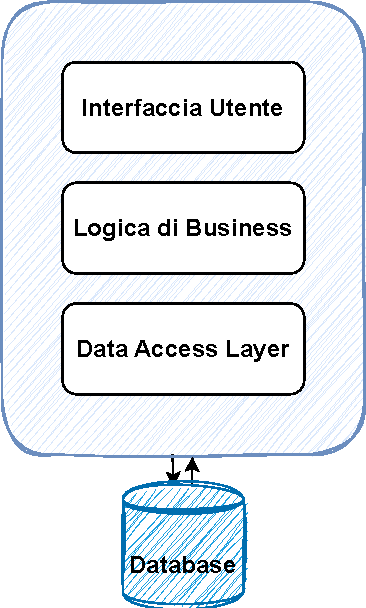
\includegraphics[scale = 0.65]{capitoli/immagini/01_architettura_monolitica.pdf}
    \caption{Architettura Monolitica}
    \label{fig:architettura_monolitica}
\end{figure}

Tale approccio nell'epoca moderna è diventato obsoleto, non è più possibile rilasciare pochi aggiornamenti annuali, che spesso risultano essere solo lavori di manutenzione, con la crescente competizione nel settore, non sviluppare ed integrare nuove funzionalità tende a far perdere interesse verso l'applicativo. L'idea di avere un'applicazione coesa in alcuni casi impone delle limitazioni non indifferenti, per esempio se il servizio di registrazione di un e-commerce non è disponibile per qualche motivo, il resto dell'applicativo deve continuare a funzione, gli utente devono poter cercare prodotti da acquistare e se già registrati, anche di poterli acquistare.

Alcuni degli approcci moderni allo sviluppo di applicazioni sono i seguenti:
\begin{enumerate}
    \item Architettura su più livelli;
    \item Architettura guidata dagli eventi;
    \item Architettura basata sui Microservizi;
\end{enumerate}

\subsection{Architettura su più livelli}
L'architettura su più livelli ha una struttura tradizionale che permette di dividere l'applicazione in diversi livelli che comunicano tra di loro. Un esempio in letteratura è il pattern \ac{MVC}, basato su tre livelli ed utilizzato spesso per lo sviluppo di applicazioni per il web. 

\begin{figure}[h]
    \centering
    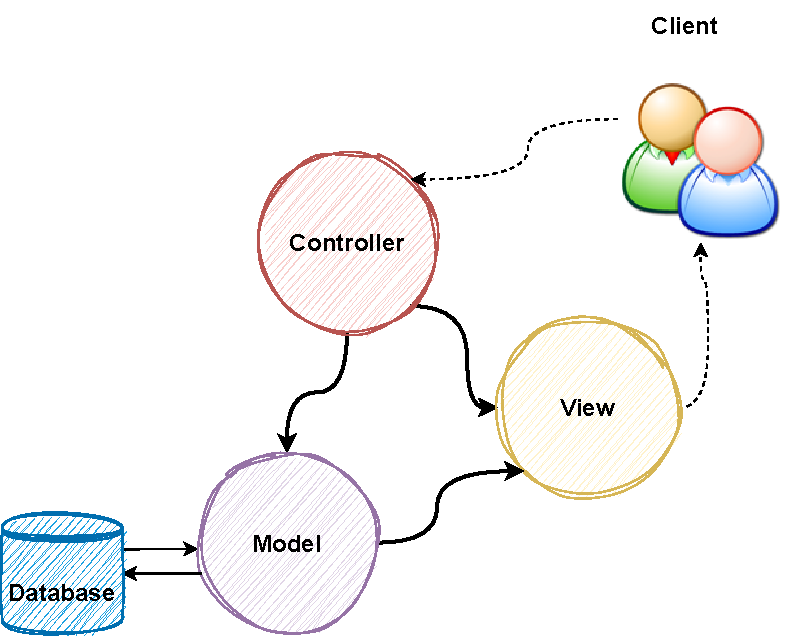
\includegraphics[scale = 0.65]{capitoli/immagini/02_pattern_mvc.pdf}
    \caption{Pattern Model-View-Controll}
    \label{fig:pattern_mvc}
\end{figure}

La suddivisione in livelli permette di semplificare la gestione delle dipendenze e l'esecuzione di funzioni logiche.

\subsection{Architettura guidata dagli eventi}
L'architettura guidata dagli eventi \cite{Event_Drive} è uno stile architetturale dove l'acquisizione, la comunicazione, l'elaborazione e la persistenza degli eventi costituiscono i pilastri portanti della soluzione.

Il fulcro di tale architettura sono gli eventi, per evento si intende qualsiasi avvenimento che porta ad un cambiamento di stato del software o dell'hardware.

L'adozione di tale architettura per la propria applicazione permette di creare un sistema più flessibile che può trasformarsi in base agli eventi, anche in tempo reale. Questo tipo di architettura è il cuore pulsante delle applicazioni sviluppate per l'\ac{IOT} che basa le proprie operazioni sull'acquisizione di dati del mondo reale, come per esempio la temperatura di una stanza o dell'umidità nell'aria, il cambiamento di un parametro che viene monitorato, porta il sistema a reagire di conseguenza.

\begin{figure}[h]
    \centering
    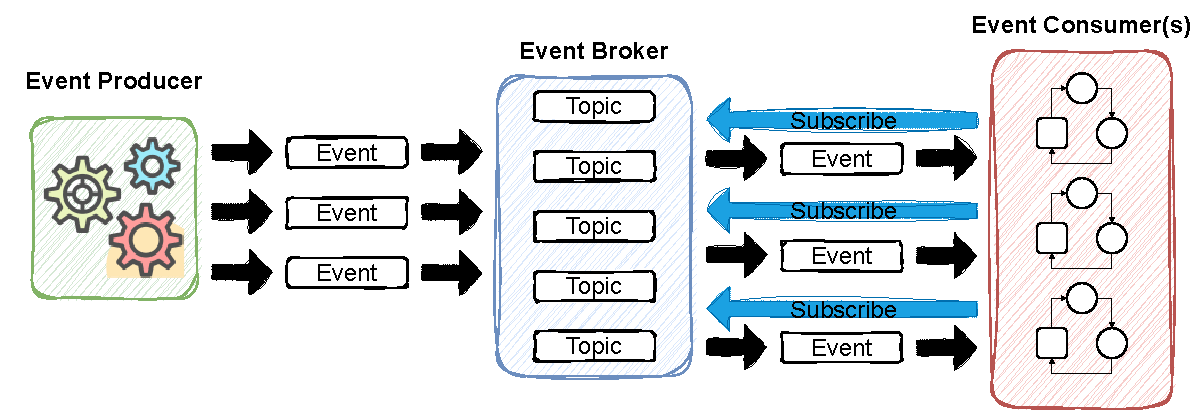
\includegraphics[scale = 0.65]{capitoli/immagini/03_architettura_guidata_dagli_eventi.pdf}
    \caption{Architettura guidata dagli eventi}
    \label{fig:architettura_event_driven}
\end{figure}

\subsection{Architettura basata sui Microservizi}
L'architettura a microservizi descrive un approccio allo sviluppo di software. Tale modello permette di scomporre le applicazioni in diversi componenti, chiamati appunto microservizi, che risultano essere indipendenti l'uno dall'altro. Ogni componente del sistema si occuperà di servire una singola funzionalità.

\begin{figure}[h]
    \centering
    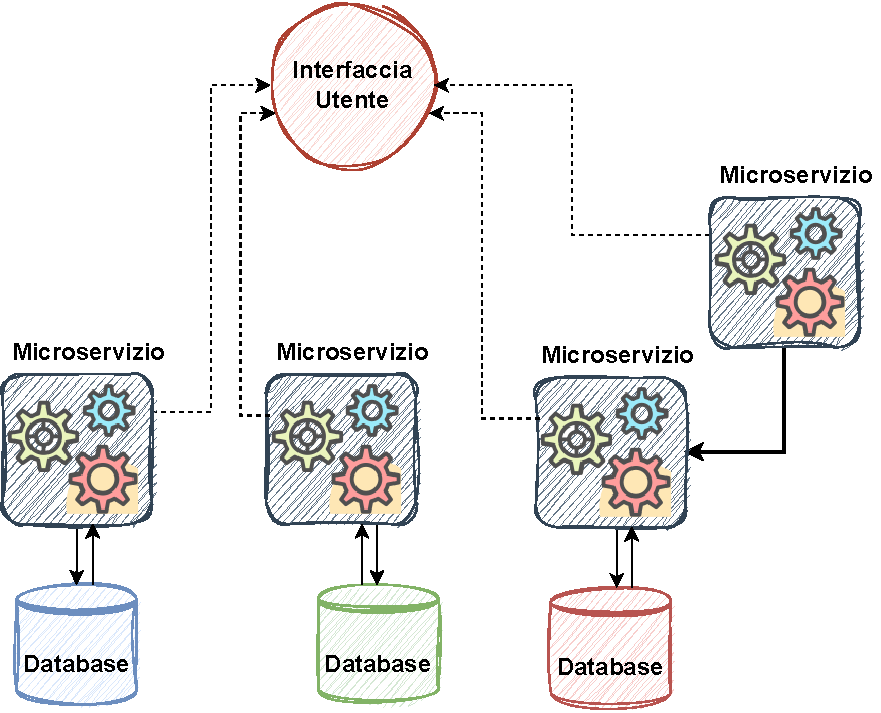
\includegraphics[scale = 0.65]{capitoli/immagini/04_architettura_microservizi.pdf}
    \caption{Architettura a microservizi}
    \label{fig:architettura_microservizi}
\end{figure}

Creando un sistema che si basa sull'approccio ai microservizi, rende la fase di manutenzione dell'applicativo più semplice, permettendo di aggiornare servizi già presenti o di sviluppare e rilasciare nuove funzionalità in un breve lasso di tempo rispetto, per esempio, all'approccio monolitico, che ricordiamo prevede pochi aggiornamenti annuali. Quello di cui abbiamo appena discusso non è l'unico vantaggio, la scalabilità dell'applicazione diventa dinamica, permettendo di gestire in autonomia il carico di lavoro. Il problema del singolo punto di vulnerabilità (Single Point of Failure) viene risolto dalla indipendenza dei microservizi, quando un componente non è disponibile per manutenzione, anomalie o altro, il sistema continuerà ad essere raggiungibile ed utilizzabile dagli utenti.



\begin{comment}
\section{Cloud Computing e Pay As You Go}
Come conseguenza dell'evoluzione della metodologia di sviluppo, ma soprattutto di come è cambiato l'approccio dei clienti, il cloud computing è diventato sempre più presente nella vita di tutti i giorni. La fisiologia alla base del cloud computing si basa sul \ac{PAYG}, non si paga più il software per ricevere una licenza full time oppure un abbonamento come nel caso dei software professionali sviluppati da Adobe (per esempio Adobe Photoshop), ma si paga solo quando il servizio è utilizzato. Un'analogia molto utilizzata per spiegare come funziona questo approccio è pensare alle utenze casalinghe, la corrente elettrica e il gas cittadino venogno pagati in base all'uso in un periodo, se, giustamente, si usa una delle due utenze o entrambe poco, si pagherà di meno rispetto a chi nello stesso periodo ha consumato molto di più.
\end{comment}


\section{Obiettivi}
L'obiettivo di questo lavoro di tesi è quello di esplorare diverse tecnologie che negli ultimi anni si stanno diffondendo, per sviluppare una semplicissima applicazione basata sull'architettura a microservizi, una sorta di Hello World che rappresenta i canoni del modello.

\section{Struttura della Tesi}
La tesi è divisa in quattro capitoli, quello appena concluso ha permesso al lettore di avere una panoramica sull'evoluzione delle architetture utilizzate nello sviluppo di software e del perché è stato necessario allontanarsi dal classico approccio monolitico. Nel prossimo capitolo andremmo ad analizzare e ad esplorare alcuni concetti teorici su cui le tecnologie utilizzate nello sviluppo odierno si basano. Il capitolo tre presenterà le tecnologie che sono state utilizzate per la creazione del software e infine, nel capitolo quattro ci concentreremo sul software sviluppato e sui punti di forza.

Il codice sorgente dell'applicazione è disponibile al seguente link: \url{https://github.com/laurus96/Microservices-Example}
\chapter{Concetti Teorici}
\section{Introduzione}
In questo capitolo vengono illustrati i concetti teorici su cui alcune tecnologie, utilizzate per la realizzazione dell'hello world, si basano.

\section{DevOps}
\subsection{DevOps e Microservizi}
Come discusso nel precedente capitolo, i microservizi sono un approccio architetturale che permette di frammentare il software in sviluppo, in piccole componenti che hanno il compito di fornire una singolà attività. L'approccio DevOps \cite{7458761} fornisce gli strumenti necessari per la gestione, lo sviluppo e la distribuzione delle applicazioni basate sui microservizi.

Data la natura dell'architettura che stiamo presentando non tutte le componenti devono essere sviluppate o integrate da noi, è possibile fare affidamento ai servizi cloud, più in generale si tende a non sviluppare componenti che magari sono già disponibile e pronti all'uso, sia per minimizzare il tempo di sviluppo, sia per concentrare tutte le forze del team sulle componenti principali del software. Fare affidamento ad un servizio cloud permette anche di semplificare la manutenzione della componente che vogliamo integrare nel nostro sistema, perché non è più compito nostro curare il servizio.

Ogni servizio però, mantiene le proprie dipendenze e questo crea un problema di integrazione, grazie alla metodologia DevOps sono stati resi disponibili diversi software per far fronte a questa problematica. Oltre al consueto utilizzo di Git per il controllo della versione, di seguito sono riportati alcuni software più diffusi e più utilizzati in questo ambito \cite{Strumenti_di_DevOps}:

\begin{table}[h]
    \centering
     \begin{tabular}{| c | c |} 
     \hline
     Automazione & \ac*{CI/CD}\\ [0.5ex]
     \hline
     Jenkins & CircleCI \\
     Docker & Bamboo \\
     Puppet & TeamCity \\
     Apache Maven & Travis CI \\
     Gradle & Buddy \\
     \hline
     \end{tabular}
    \caption{Strumenti per l'automazione e CI/CD}
    \label{tab:table1}
\end{table}

\begin{table}[h]
    \centering
     \begin{tabular}{| c | c | c | c |} 
     \hline
     Configurazione & Testing & Monitoraggio\\ [0.5ex]
     \hline
     Chef & Selenium & Nagios \\
     Kubernetes & Tricentis Tosca & Prometheus \\
     Ansible & TestSigma & New Relic \\
     Vagrant & IBM Rational Functional & PagerDuty \\
     Consul & SoapUI & Sensu \\
     Terraform &  & Splunk \\
     & & ELK Stack \\
     \hline
     \end{tabular}
    \caption{Strumenti per la configurazione, testing e monitoraggio}
    \label{tab:table2}
\end{table}


\section{Container Linux}
I Container \cite{Container_Linux} sono una tecnologia già apparsa nei primi anni 2000. Nel sistema operativo FreeBSD era presente una funzione chiamata jail, prigione, ed era uno strumento per isolare una porzione del sistema operativo. Tale tecnologia è stata implementata in GNU/Linux dal 2001 e con le varie implementazioni e le varie migliorie sono nati i container, degli spazi del sistema operativo sicuri e controllati.

In Linux il loro funzionamento viene gestito dai cgroups\footnote{Gruppi di Controllo}, strumenti che operano a livello kernel e che permettono di limitare le risorse utilizzate da un processo o da un gruppo di processi. I gruppi di controllo usano systemd che permette di inizializzare i processi ed isolarli dal resto del sistema operativo.

Attualmente i container sono un approccio utilizzato sia in ambito di sviluppo che in ambito di rilascio e sono nati diversi software per la loro gestione come Linux Container Daemon (comunemente chiamato LXD), Podman e Docker.

\begin{figure}[h]
    \centering
    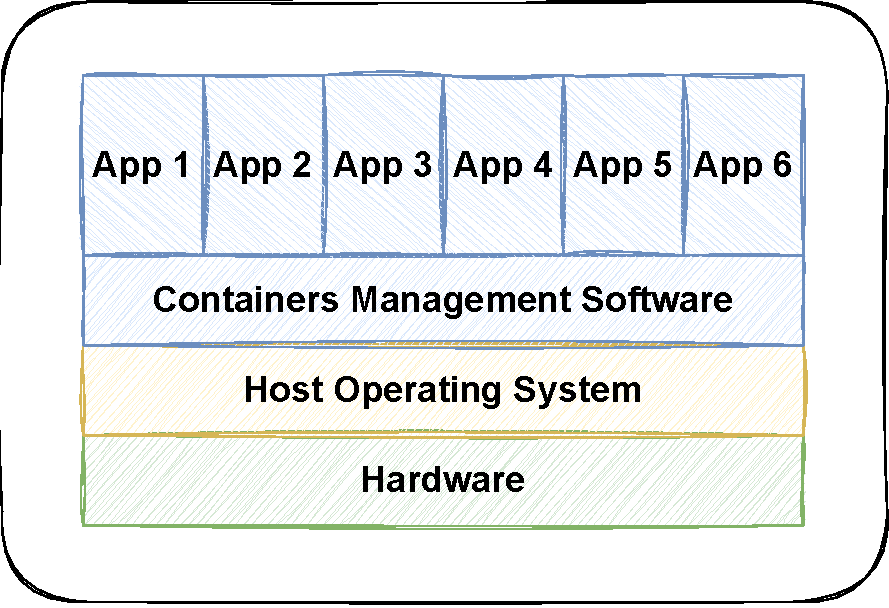
\includegraphics[scale=0.65]{capitoli/immagini/05_container_architecture.pdf}
    \caption{Architettura per la gestione dei container}
    \label{fig:container_architecture}
\end{figure}

\subsection{Macchine Virtuali}
I container vengono molto spesso scambiati per una tipologia di macchina virtuale, questo avviene in maniera errata, perché come abbiamo visto nel paragrafo precedente, i container rappresentano una porzione del sistema operativo creata e gestita da strumenti che lavorano a livello kernel del sistema operativo GNU/Linux. 

Per definizione invece una macchina virtuale crea un ambiante virtuale dove si cerca di emulare il comportamento di una macchina fisica, quindi si cerca non solo di emulare il funzionamento del sistema operativo, ma anche dell'hardware sottostante.

Container e macchine virtuali, seppur diversi per definizione, vengono usati molto spesso per raggiungere lo stesso scopo, quello di rilasciare un software già configurato e pronto all'uso. Per questo motivo ci sono molti lavori che mettono a confronto le due tecnologie come nel caso del lavoro \cite{seo2014performance} di Seo, Kyoung-Taek and Hwang, Hyun-Seo and Moon, Il-Young and Kwon, Oh-Young and Kim, Byeong-Jun che ci permette di osservare come l'utilizzo dei container fornisca delle performance migliori (in questo particolare caso) rispetto all'utilizzo di una macchina virtuale. Questo però non significa che le macchine virtuali ad oggi sono uno strumento datato o superato.

\begin{figure}[h]
    \centering
    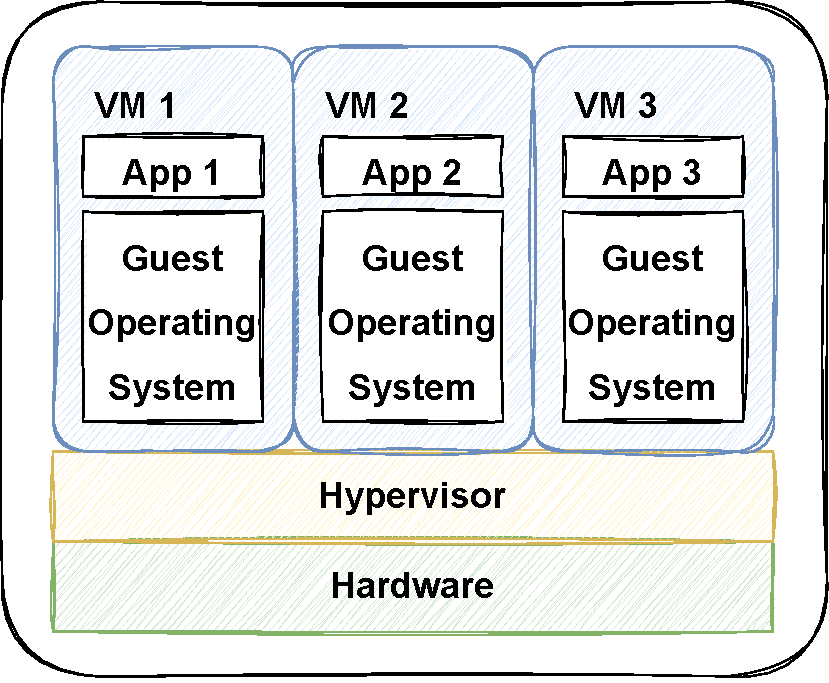
\includegraphics[scale=0.65]{capitoli/immagini/06_virtual_machine_architecture.pdf}
    \caption{Architettura per la gestione di macchine virtuali}
    \label{fig:vm_architecture}
\end{figure}

\subsection{Immagine di un container}
Abbiamo già visto come è definito un container, ora ci chiediamo come sia possibile usare tale tecnologia. I software per la gestione dei container supportano un particolare tipo di file che fornisce agli strumenti che si occupano della creazione del container, importanti schemi di configurazione. Tale file è chiamato immagine di container e rappresenta, in via astratta, quella porzione del sistema operativo che contiene la nostra applicazione con tutte le dipendenze soddisfatte, tutte le configurazioni, gli script e altro.

Le immagini dei container ci permettono di condividere tale applicazioni con altri utenti e di poterle installare con facilità. Ogni programma di gestione dei container definisce il proprio standard di creazione delle immagini.

Di solito le immagini vengono caricate in un  registro, chiamato comunemente container registry, uno spazio dedicato all'archiviazione dell'immagine dove è possibile gestirle ed avere strumenti utili per l'analisi, per esempio alcuni container registry offrono il servizio di analisi delle vulnerabilità.

\subsection{Orchestrazione dei Container}
Ripensando alla definizione data in precedenza per l'architettura a microservizi e applicando a tale definizione la tecnologia appena presentata, possiamo osservare come ogni componente del nostro sistema può essere considerato come un container, in fondo, abbiamo ripetuto più volte che un microservizio è un'entità autonoma e indipendente, e un container, per definizione, è una porzione di sistema operativo isolato (attenzione questo non implica che i container non possano dialogare tra di loro). La nostra applicazione sarà costituita alla fine da tanti container. Data la necessità di dover gestire più container alla volta, sono \cite{burns2022orchestrazione} nati software che si occupano proprio di questo aspetto. 

In generale questo tipo di software creano uno strato aggiuntivo tra l'applicativo che si occupa dei container e i container veri e propri:

\begin{figure}[h]
    \centering
    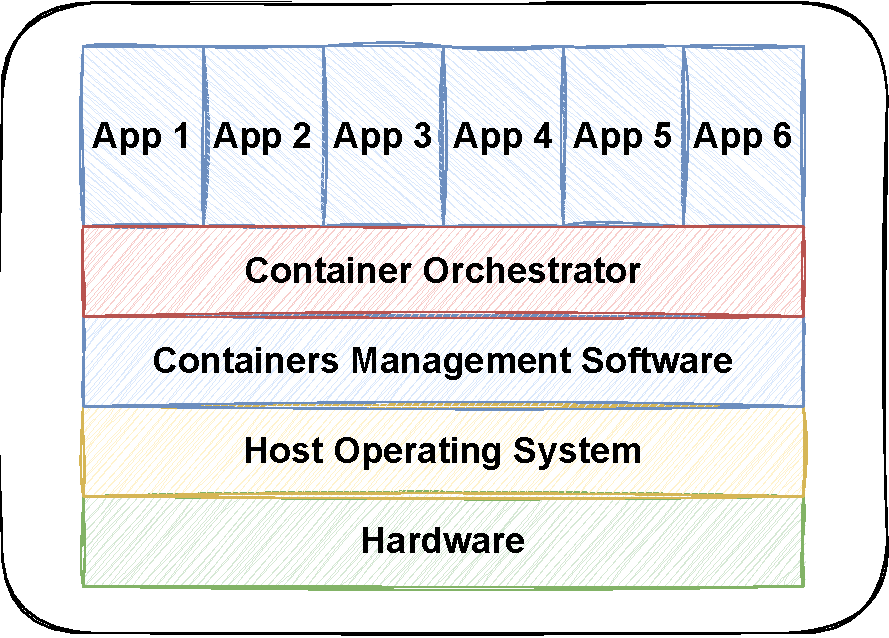
\includegraphics[scale=0.65]{capitoli/immagini/07_container_architecture_orchestrator.pdf}
    \caption{Architettura con software per l'orchestrazione dei container}
    \label{fig:orchestrator}
\end{figure}


Software per l'orchestrazione dei container \cite{cabibbo2022orchestrazione} mettono a disposizione strumenti in grado di eseguire diverse operazioni di gestione, come il monitoraggio dello stato, il carico di lavoro attuale e molto altro.


\section{Lato backend di un applicativo}
Di solito possiamo dividere le nostre applicazioni in due grandi blocchi chiamati rispettivamente backend e frontend. La parte backend di un'applicazione implementa la cosidetta logica di business, mentre la parte di frontend rappresenta ciò che è visibile all'utente finale.

Nel corso degli anni sono nate diverse tecnologie per lo sviluppo e la gestione di questi macro blocchi e con la crescente complessità delle applicazioni sono nati anche dei software utili per gestire e risolvere diversi problemi che appaiono nei grandi progetti, come la gestione delle dipendenze.

Secondo le principali piattaforme di ricerca per il lavoro i linguaggi più popolari per lo sviluppo back end sono: Java, Python, C\# e JavaScript e stanno crescendo l'uso di Rust e Golang.
Di seguito è riportata una tabella con i principali framework assegnati al linguaggio di programmazione:

\begin{table}[h]
    \centering
    \begin{tabular}{| c | c |}
        \hline
       Linguaggio di Programmazione  &  Framework  \\
       \hline
       Java  & Springboot \\
       C\# & ASP.NET \\
       JavaScript & Node.js \\
       Python & Django \\
       \hline
    \end{tabular}
    \caption{Framework associato al proprio linguaggio di programmazione}
    \label{tab:backend_framework}
\end{table}

\subsection{Gestione delle dipendenze}
Una delle problematiche che affligge i gradi progetti è la gestione delle dipendenze. Molto spesso in applicativi reali si tende ad utilizzare diverse tecnologie per rispettare standard o per utilizzare funzioni che il linguaggio di programmazione scelto non rende disponibili tramite le librerie di base. Negli anni sono nati degli strumenti che permettono di automatizzare la gestione delle dipendenze delegando ad un software tutto il lavoro necessario per installare, aggiornare e gestire nuove dipendenze.

\begin{comment}
\subsection{Framework per backend}
Come in ogni altro campo l'avanzamento tecnologico ha portato alla creazione di diverse tecnologie per semplificare lo sviluppo. Anche linguaggi nati principalmente per l'uso in front end hanno visto la creazione di strumenti di framework per lo sviluppo in back end. I linguaggi di programmazione più popolari per lo sviluppo back end secondo le principali piattaforme di ricerca del lavoro sono: Java, Python, C\# e JavaScript e stanno crescendo l'uso di Rust e Golang.

Di seguito è riportata una tabella con i principali framework assegnati al linguaggio di programmazione:

\begin{table}[h]
    \centering
    \begin{tabular}{| c | c |}
        \hline
       Linguaggio di Programmazione  &  Framework  \\
       \hline
       Java  & Springboot \\
       C\# & ASP.NET \\
       JavaScript & Node.js \\
       Python & Django \\
       \hline
    \end{tabular}
    \caption{Framework associato al proprio linguaggio di programmazione}
    \label{tab:backend_framework}
\end{table}
\end{comment}


\chapter{Tecnologie nel dettaglio}
\section{Introduzione}
In questo capitolo andremo ad introdurre e analizzare alcune tecnologie che implementano i concetti riportanti nel capitolo precedente. Lo scopo di questo capitolo è quello di permettere al lettore di familiarizzare con alcuni concetti che poi saranno trattati nel prossimo capitolo.

\section{Gestione dei container: Docker}
Uno dei software disponibili per la gestione dei container, nonché uno dei più famosi, è Docker. Disponibile in forma gratuita, Docker è un progetto open source scritto interamente in Go e supportato da numerose aziende, come Google.

Abbiamo già discusso riguardo alla funzionalità e alla potenzialità dei container nel precedente capitolo. Grazie a Docker è possibile utilizzare i container anche su macchine che non utilizzano il kernel di GNU/Linux, in queste macchine viene creato uno strato aggiuntivo di virtualizzazione che permette all'applicativo di creare e gestire i container. Docker fornisce agli sviluppatori gli strumenti necessari per creare, gestire e configurare i container, tramite linea di comando o tramite un'interfaccia grafica.

\subsection{L'architettura di Docker}
L'architettura di Docker è basata sul tradizionale modello client-server.

\begin{figure}[h]
    \centering
    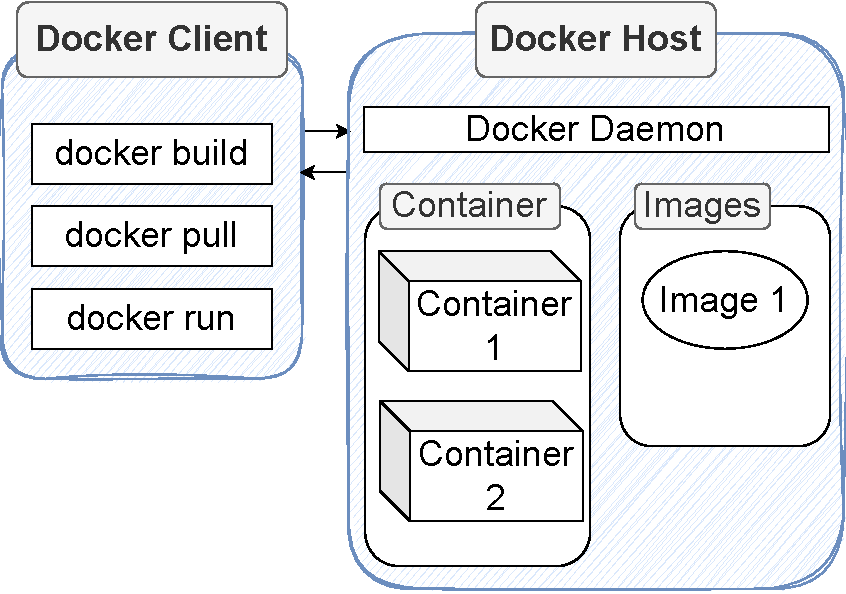
\includegraphics[scale=0.65]{capitoli/immagini/08_docker_architecture.pdf}
    \caption{Architettura di Docker}
    \label{fig:docker_arch}
\end{figure}

\paragraph{Docker Client}
Il docker client permette all'utente di interagire tramite interfaccia grafica o tramite riga di comando con il docker host. L'interfaccia grafica implementata in Docker però non permette di gestire tutte le componenti, l'utilizzo di Docker tramite riga di commando è consigliato anche dalla documentazione ufficiale. Di seguito sono riportati alcuni dei comandi più frequentemente usati:

\begin{enumerate}
    \item \textbf{\textcolor{color_1}{docker build -t <image\_name>}};
    \item \textbf{\textcolor{color_1}{docker pull <image\_name>}};
    \item \textbf{\textcolor{color_1}{docker run --name <container\_name> <image\_name>}};
\end{enumerate}

Il primo comando permette di creare un'immagine da un dockerfile \footnote{Un file di configurazione usato da Docker per la creazione di immagini.}, il secondo di scaricare un'immagine da Docker Hub \footnote{Il container register ufficiale di Docker \url{https://hub.docker.com/}.}. Il terzo comando permette la creazione di un container da un'immagine presente in locale, nel caso l'immagine non sia presente, Docker avviserà l'utente che dovrà eseguire il comando due per scaricare l'immagine richiesta.


\paragraph{Docker Host}
Il docker host rappresenta il cuore di Docker. Questo componente ha il compito di controllare i container. Per la definizione data in precedenza sappiamo che un container rappresenta una porzione del sistema operativo completamente isolata, allora ci chiediamo come sia possibile che i container, nella realtà, riescano a connettersi e scambiari informazioni tra di loro. Il kernel GNU/Linux non fornisce nessun meccanismo di dialogo tra container, ma Docker implementa una logica di networking per eliminare questo limite. L'implementazione delle regole di networking però rende le applicazioni che utilizzano i container meno sicure, durante la fase di sviluppo bisogna tener conto delle vulnerabilità scoperte sulle tecnologie utilizzate e correggerle. Per questo alcuni registri delle immagini permettono di effettuare delle scansioni sulle immagini e in caso di vulnerabilità notificare l'utente.

Di base tutti i file generati all'interno di un container vengono archiviati momentaneamente in un layer di persistenza dei dati, una volta che il container verrà distrutto (o terminato), i dati creati andranno perso. Docker implementa un meccanismo per rendere la persistenza dei dati definitiva, andando ad affidarsi alla macchina su cui docker host è in esecuzione. 

\begin{figure}[h]
    \centering
    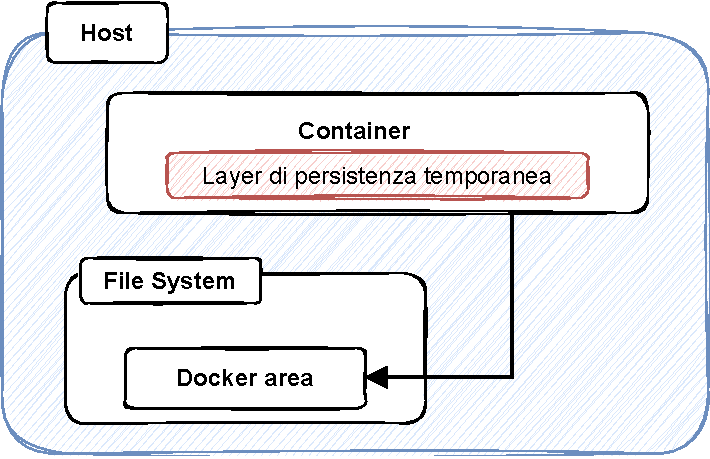
\includegraphics[scale=0.65]{capitoli/immagini/09_docker_volume.pdf}
    \caption{Persistenza dei dati in Docker}
    \label{fig:docker_persistance}
\end{figure}

Per semplicità consideriamo che Docker sia installato su una distribuzione del sistema operativo GNU/Linux, come possiamo osservare dalla figura sopra riportata, Docker implementa un meccanismo che permette ai container di dialogare col file system del computer host per accedere ad un'area di memoria, denominata docker area e creata durante l'installazione di Docker, e rendere persistenti i file creati durante l'esecuzione del container \footnote{In realtà Docker implementa altri due sistemi per la persistenza dei dati, il primo salva i dati generati in una qualsiasi posizione libera della memoria del computer host, il secondo metodo invece permette di depositare i dati nella memoria centrale, di fatto rendendoli temporanei.}. 

\section{Orchestrazione dei Container: Kubernetes}
Kubernetes \cite{K8S} è un software per l'orchestrazione dei container open source che  fornisce gli strumenti necessari per gestire i sistemi distribuiti in modo resiliente. Uno degli strumenti più importanti che Kubernetes implementa è il load balancer, alcune volte può presentarsi un eccessivo carico di lavoro su uno dei servizi, il load balancer permette una gestione automatica del carico di lavoro, in modo da non causare anomalie nel sistema.

Kubernets è un software che generalmente è disponibile tramite un servizio cloud, quando richiediamo un servizio del genere ciò che ci viene assegnato è chiamato un cluster. Di seguito possiamo osservare come funziona un cluster di Kubernetes:

\begin{figure}[h]
    \centering
    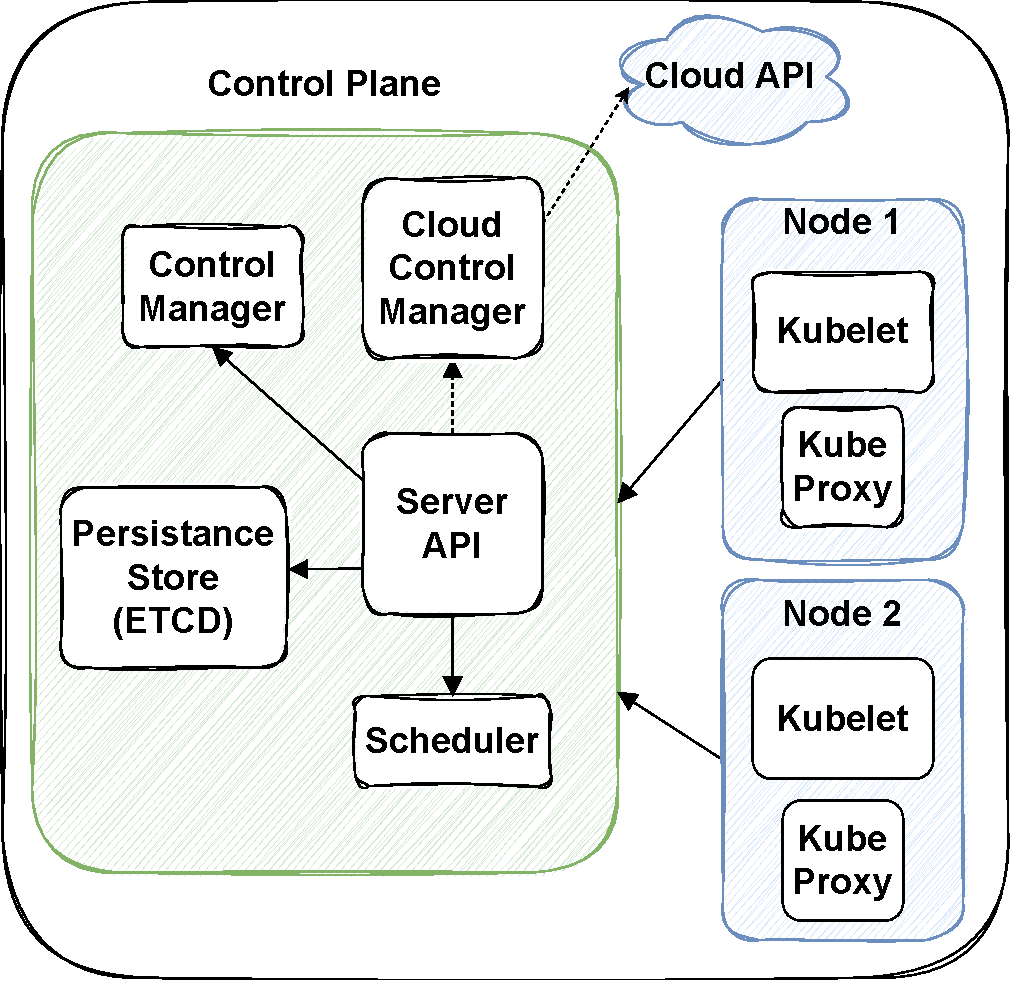
\includegraphics[scale=0.65]{capitoli/immagini/10_cluster_kubernetes.pdf}
    \caption{Cluster Kubernetes}
    \label{fig:Kubernetes_Cluster}
\end{figure}

\begin{comment}
\begin{itemize}
    \item Scoperta dei servizi e bilanciamento del carico;
    \item Orchestrazione dello storage; 
    \item Rollout e rollback automatizzati;
    \item Ottimizzazione dei carichi;
    \item Self-healing;
    \item Gestione di informazioni sensibili e della configurazione;
\end{itemize}
\end{comment}


\paragraph{Control Plane}
Il control plane è il componente principale di ogni cluster, mette a disposizione dell'utente tutte le funzionalità principali di Kubernetes. Il control plane può anche essere distribuito su più macchine.

\paragraph{Server API}
La prima componente che approfondiamo è il Server API. Il compito di questo componente è quello di esporre le API per accedere al control plane e poter controllare lo stato l'intero cluster. 

\paragraph{Persistance Store}
ETCD\footnote{Letteralmente /etc distributed.} è un software open source che si basa su concetto di rendere distribuita la cartella /etc presente nei sistemi operativi basati su Unix. In Unix la cartella etc contiene diversi file di configurazione. La componente integrata nel cluster di Kubernetes si occupa di rendere persistenti i file di configurazione utilizzando un sistema di chiave-valore e creando automaticamente dei backup sui dati ogni 30 minuti.

\paragraph{Scheduler}
Lo scheduler è quel componente del cluster che si occupa di gestire i nuovi pods assegnandoli ad uno dei nodi disponibile. Per pod si intende un gruppo di uno o più container che condividono le stesse informazioni di networking e di persistenza dei dati. Un pod rappresenta la più piccola unità che può essere creata e gestita da Kubernetes.

\paragraph{Controller Manager}
Il controller manager è formato da un insieme di processi che si occupano di gestire diverse parti del cluster. Un controller è un componente che  monitora costantemente lo stato del cluster tramite il server api e se lo stato desiderato non è quello attuale cerca di riportare il sistema ad uno stato precedente.

\paragraph{Cloud Controller Manager}
Esattamente come il controller manager, il cloud controller manager rappresenta un insieme di processi controller che si occupano di monitorare lo stato del cluster, ma solo di quelle componenti che gestiscono i processi cloud. Il cloud controller manager crea un collegamento tra il server API e la piattaforma di cloud scelta. Se per esempio si sceglie di utilizzare Kubernetes senza fare affidamento ad un servizio di cloud esterno, questa componente non farà parte del cluster.

\paragraph{Node}
Un nodo rappresenta un ambiente di runtime dove i container sono creati e gestiti.

\paragraph{Kubelet}
Processo che gestisce l'esecuzione dei container nei pod. Tale componente prevede l'esecuzione di diverse istruzioni che monitorano lo stato dei pod.

\paragraph{Kube-Proxy}
La rete condivisa tra container dello stesso pod viene gestita dalla componente nota come kube-proxy, inoltre permette ad un nodo di poter dialogare con gli altri nodi del cluster. L'implementazione base prevede l'utilizzo delle regole di networking del sistema operativo, ma è anche possibile che sia stesso la componente a gestire le comunicazioni.

\subsection{Orchestrazione in locale: minikube}
Kuberntes è un servizio accessibile principalmente via un servizio cloud. Generalmente tutti i più grandi cloud provider permettono di instanziare un cluster di Kubernetes. Essendo Kubernetes un software open source, la community ha reso disponibile un'implementazione in locale chiamata minikube. Tale software utilizza proprio Docker per emulare il funzionamento di Kubernetes.

\section{Gestione del Progetto: Apache Maven}
Una delle problematiche che affligge lo sviluppo moderno è la gestione delle dipendenze. Durante lo sviluppo di applicazioni è necessario fare affidamento su librerie esterne, per sopperire a mancate implementazione del linguaggio utilizzato. Una delle librerie esterne più utilizzate per lavorare con i file \ac{JSON} in Java è la libreria sviluppata da Google e mantenuta dalla comunità open source GSON. Java permette l'uso di librerie esterne a patto che il loro file sia incluso nel progetto. L'inclusione manuale delle librerie in Java però porta a diverse problematiche, sia con le librerie stesse, sia col coordinamento con il team di sviluppo, se il nostro progetto necessitasse di più librerie esterne dovremmo scaricare da Internet il file e poi includerlo nel nostro progetto e per ogni libreria dovremmo soddisfare, se presente, la catena di dipendenze, nel fare questo dovremmo anche informare il resto del team di sviluppo. 

Fortunatamente sono stati sviluppati software che si occupano di questo particolare aspetto (e non solo) della gestione del progetto. Apache Maven è uno di questi software ed è utilizzato principalmente in applicativi software basati su Java. Grazie a Maven la gestione delle dipendenze di un progetto diventa molto più semplice.

Maven non è uno strumento che gestisce solo le dipendenze di un progetto, permette anche di automatizzare la creazione del pacchetto e la possibilità di specificare una determinata struttura di progetto.

Il fulcro del software è un file chiamato \ac{POM}, scritto in \ac{XML}, tale file contiene tutte le istruzioni che necessità Maven per una corretta gestione del progetto. Nel pom sono presenti diverse informazioni, quelle più generiche che riguardano la versione, il nome, le informazioni sulla versione di Java utilizzata o altro, a quelle più specifiche come le dipendenze da soddisfare per il corretto funzionamento del software in sviluppo.

Maven permette anche di integrare dei plugin di terze parti, in questo modo è possibile creare degli strumenti per personalizzare il comportamento di Maven. Per esempio il framework Spring Boot integra il proprio plugin all'interno dei suoi progetti che utilizzano Maven.

\subsection{Un esempio di POM}

\paragraph{Introduzione del file}
Le prime righe di ogni file pom specificano la  versione della struttura e delle specifiche da seguire per quanto riguarda la scrittura dell'intero documento.
\begin{lstlisting}[language=XML, caption=Introduzione del POM]
<?xml version="1.0" encoding="UTF-8"?>
<project xmlns="http://maven.apache.org/POM/4.0.0"
	xmlns:xsi="http://www.w3.org/2001/XMLSchema-instance"
	xsi:schemaLocation="http://maven.apache.org/POM/4.0.0 https://maven.apache.org/xsd/maven-4.0.0.xsd">
	<modelVersion>4.0.0</modelVersion>
\end{lstlisting}


\paragraph{Informazioni del progetto}
Dopo le informazioni che riguardano il documento xml, abbiamo le informazioni che riguardano il progetto vero e proprio. 
\begin{lstlisting}[language=XML, caption= Informazioni del progetto che Maven deve gestire]
	<groupId>com.example.package</groupId>
	<artifactId>package</artifactId> <!-- Nome del pacchetto JAR/WAR -->
	<version>0.0.1-SNAPSHOT</version> <!-- Versione del pacchetto JAR/WAR -->
	<name>Nome del progetto</name>
	<description>Descrizione</description>
\end{lstlisting}
Come è possibile leggere in questa parte di xml vengono specificate le informazioni come nome del progetto, versione e descrizione. Queste informazioni sono utili a Maven durante la fase di creazione del pacchetto. Possono anche essere specificate delle proprietà, come per esempio la versione di Java utilizzata:
\begin{lstlisting}[language=XML, caption= Specifica della versione di Java]
	<properties>
		<java.version>11</java.version>
	</properties>
\end{lstlisting}


\paragraph{Dipendenze e Plugin}
Infine, il cuore del pom contiene tutte le informazioni per la gestione delle dipendenze e dei plugin. In questa parte di codice oltre a specificare quali plugin e quali dipendenze si intende utilizzare è anche possibile specificare ulteriore regole che Maven dovrà eseguire. Per esempio nei progetti in Java viene quasi sempre utilizzato il framework JUnit per effettuare dei test sull'applicativo in fase di sviluppo, questo pacchetto però non sarà più necessario quando l'applicazione sarà pronta per la distribuzione ed è possibile definire delle regole per escludere la dipendenza di JUnit quando Maven si occuperà di creare il pacchetto destinato al rilascio.
\begin{lstlisting}[language=XML, caption=Dipendenze e Plugin nel POM]
	<dependencies>
		<!-- Sezione dedicata alle dipendenze da soddisfare -->
	</dependencies>

	<build>
		<plugins>
			<!-- Sezione dedicata ai Plugin-->
		</plugins>
	</build>
</project>
\end{lstlisting}


\section{Framework: Spring Boot}
Uno dei framework più utilizzati per lo sviluppo back-end con il linguaggio di programmazione Java è sicuramente Spring Boot. La popolarità di questo framework lo rende una delle scelte migliori quando si decide di lavorare ad un applicazione che necessita di Java, grazie alla vasta utenza che ha deciso di includerlo nel propri progetti in rete è possibile trovare soluzioni di ogni tipo. Netflix è la principale sostenitrice del progetto Spring Boot, non solo aiuta nello sviluppo del framework, ma lo utilizza anche per il suo sistema basato sull'applicazione di streaming.

Spring Boot è basato sul framework Spring che a sua volta è basato sulle specifiche di Java Enterprise Edition. Il framework che stiamo esplorando ha 3 vantaggi principali:
\begin{enumerate}
    \item Configurazione automatica;
    \item Inversion of Control;
    \item Portabilità dell'applicativo;
\end{enumerate}

\paragraph{Configurazione automatica}
Le funzionalità implementate da Spring Boot sono operative dal momento della loro richiesta. Per esempio, se viene richiesta la componente di Spring Security, che come intuibile dal nome implementa i servizi per rendere sicura l'applicazione, una volta che la dipendenza sarà soddisfatta, Spring Boot assumerà il controllo per applicare a tale componente una configurazione di base, di fatto rendendola subito operativa.

Questo meccanismo non implica però che tale configurazione di base non possa essere modificata per implementare magari dei servizi aggiunti. Facendo riferimento sempre al caso di Spring Security, nessuno ci vieta di implementare un ulteriore sistema di autenticazione come \ac{JWT}.

Spring Boot permette di dover scrivere meno codice grazie alla configurazione automatica delle componenti, ma allo stesso tempo fornisce i meccanismi per configurare manualmente a nostro piacimento tale componente.

\paragraph{ Inversion of Control }
Il framework Spring Boot eredità da Spring due meccanismi: l'inversion of control e la dependency injection. 

Per inversion of control si intende quel meccanismo di ingegneria del software che trasferisce il controllo non più agli oggetti del nostro applicativo, ma al framework stesso. Nei linguaggi di programmazione tradizionali, come il C, noi facciamo uso delle librerie, con l'inversion of control il framework prende il controllo del flusso del nostro codice e quando richiesto lo richiama. 

I vantaggi dell'inversion of control sono diversi:
\begin{enumerate}
    \item disaccoppiamento dell'esecuzione di un servizio e la sua implementazione;
    \item facilità di implementazione di diverse soluzioni;
    \item facilità di testing dell'intero applicativo, grazie alla possibilità di isolare componenti e le loro dipendenza.
    \item una maggior modularià del programma;
\end{enumerate}
Per implementare l'inversion of control Spring utilizza il design pattern dependency injection.



\paragraph{Portabilità}
La portabilità è l'ultimo aspetto principale di Spring Boot. Questa funzionalità permette di creare un unico pacchetto con estensione \ac{WAR} del nostro applicativo, ma a differenza di un file WAR classico, Spring Boot rende il nostro pacchetto completo, pronto per il deployment.

\chapter{Hello World}

\section{Introduzione}
In questo capitolo applicheremo i concetti teorici descritti precedentemente per sviluppare un software basato sui microservizi. Lo scopo è quello di verificare come tale approccio permette uno sviluppo più semplice delle applicazioni dividendo l'intera logica di business in piccoli servizi ognuno indipendente dall'altro.


\subsection{Pom di Spring Boot}
L'utilizzo di Spring Boot come framwork back-end genera un file pom con delle informazioni di base. Queste informazioni sono condivise tra tutti i progetti che utilizzano Maven e Spring Boot.

\begin{lstlisting}[language=XML]
	<!-- ... -->
	<parent>
		<groupId>org.springframework.boot</groupId>
		<artifactId>spring-boot-starter-parent</artifactId>
		<version>2.7.5</version>
		<relativePath/> <!-- lookup parent from repository -->
	</parent>
	<!-- ... -->
			<plugin>
				<groupId>org.springframework.boot</groupId>
				<artifactId>spring-boot-maven-plugin</artifactId>
			</plugin>

\end{lstlisting}

Nel nostro caso l'estratto del pom riportato indica l'aggiunta dell'utilizzo del framwork Spring Boot alla versione 2.7.5 e l'aggiunta del plugin ufficiale sviluppato da Spring Boot.


\subsection{Struttura dei servizi}
Per la gestione dei singoli progetti abbiamo utilizzato Apache Maven. Come spiegato nei precedenti capitoli, Maven è un ottimo strumento, non solo permette di soddisfare tutte le dipendenze richieste dall'applicativo, ma permette anche di standardizzare la struttura di un progetto, per Spring Boot la struttura è molto simile ad un semplice progetto in Java. 


\begin{figure}[h!]
    \centering
    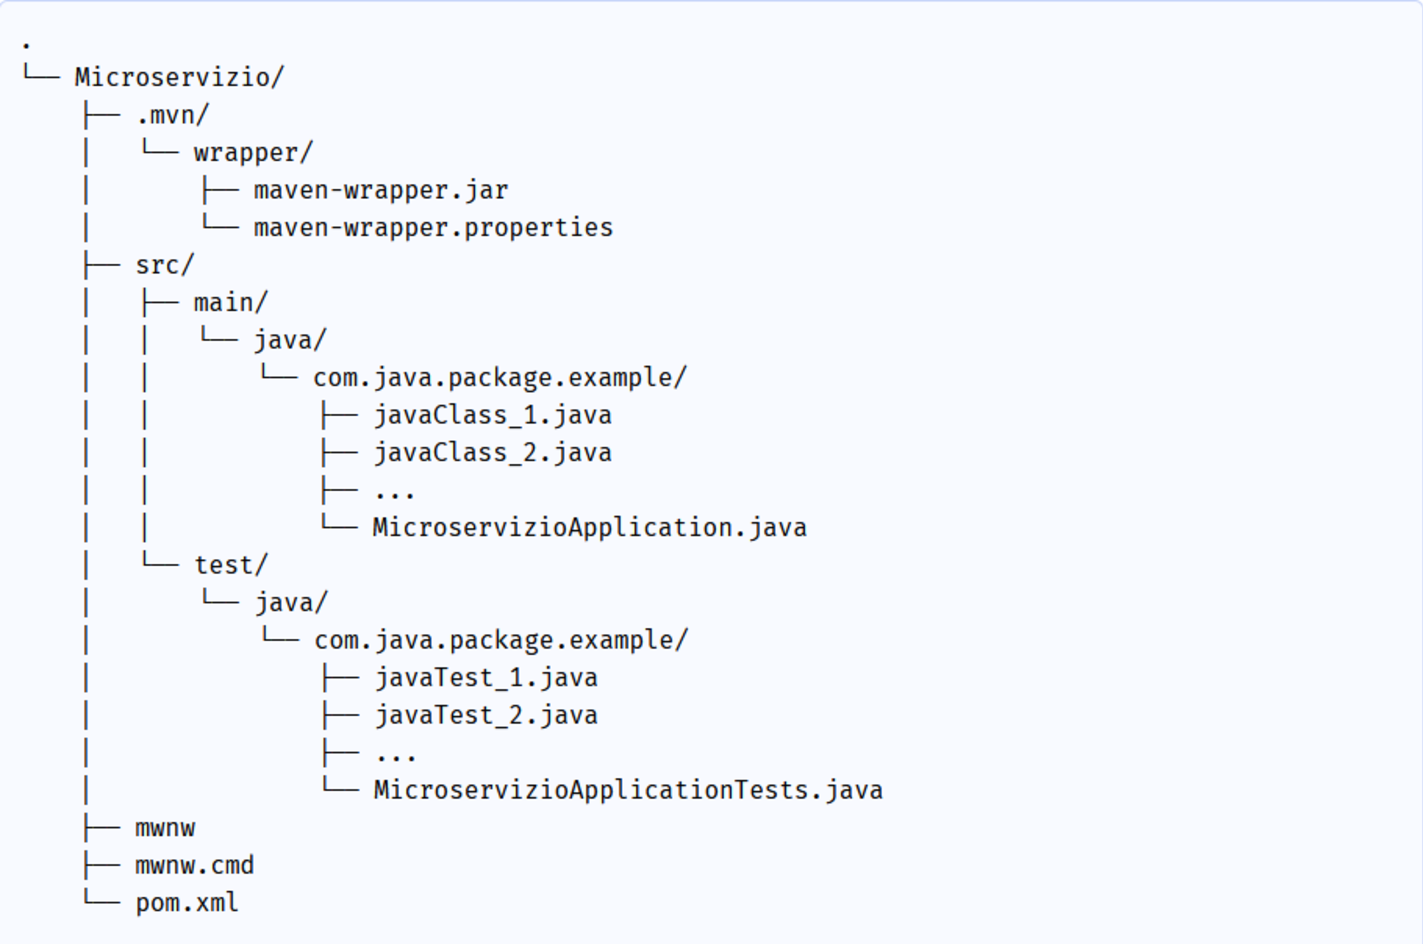
\includegraphics[scale = 0.60]{capitoli/immagini/11_maven_tree.pdf}
    \caption{Struttura per i progetti in Spring Boot}
    \label{fig:maven_structure_springboot}
\end{figure}

\section{Architettura}

L'applicazione sviluppata presenta tutta la logica di business all'interno di due microservizi. Image Service è il primo servizio sviluppato, il suo scopo è quello di recuperare delle informazioni su delle immagini. Gallery Service invece ha il compito di filtrare le varie immagini esposte dal servizio precedentemente elencato.

\begin{figure}[h]
    \centering
    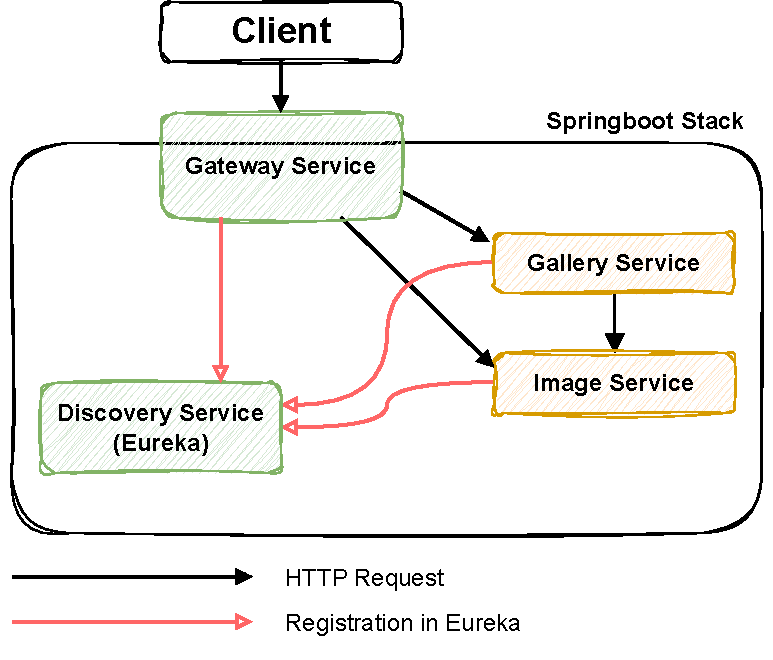
\includegraphics[scale = 0.65]{capitoli/immagini/12_architettura_hello_world.pdf}
    \caption{Architettura del software}
    \label{fig:architettura_hello_worlds}
\end{figure}

Come possiamo notare dal diagramma dell'architettura, sono riportati altri due servizi che prima non sono stati menzionati. Il gateway service ha l'obiettivo di esporre l'intera applicazione all'utente finale tramite un singolo punto di accesso. L'utente digitando l'\ac{URL} esposto dal servizio di gateway nel proprio browser, riesce ad accedere immediatamente all'applicazione, ma in realtà sarà il gateway che si occuperà di instradare i dati in entrata e in uscita.

Il discovery service è forse il più importante perché permette di gestire tutti i servizi che compongono l'applicazione, anche quelli non visibili all'utente finale. Eureka è il nome del discovery service messo a disposizione dal framework Spring Boot.




\subsection{Eureka Discovery Service}
Il servizio di scoperta si occupa di registrare tutti i servizi dell'applicazione in modo da poter esser gestiti. 

\paragraph{File di configurazione}
Il file di configurazione per i progetti che utilizzano il framework Spring Boot è denominato application.properties \footnote{In alcuni vecchi progetti o nella documentazione ufficiale è possibile trovare questo file con l'estensione yaml}. All'interno sono specificati parametri che aiutano la configurazione delle applicazioni. Nel caso del nostro servizio il file in questione è scritto in questo modo:

\begin{lstlisting}[caption=Application.properties di Eureka]
spring.application.name=eureka-server

server.port=8761

eureka.instance.prefer-ip-address=true
eureka.client.register-with-eureka=false
eureka.client.fetch-registry=false
\end{lstlisting}

Nel file sono riportate alcune informazioni base come il nome e la porta su cui verrà esposto il servizio, questo parametro andrà a sovrascrivere la configurazione base del server Tomcat che di default espone gli applicativi sulla porta 8080. dato che la nostra applicazione avrà diverse componenti conviene assegnare ad ognuno una porta diversa.

Ulteriori informazioni impostano dei parametri per il servizio eureka, in questo file specifichiamo che diamo libero arbitrio ad Eureka per quando riguarda la gestione della registrazione dell'indirizzo ip dei vari microservizi.

L'implementazione di Eureka prevede la presenza di due enti, il server e i client. Il servizio di discovery si comporta da server mentre i vari microservizi da client, quest'ultimi una volta effettuato il deploay cercheranno subito di contattare il discovery service (server) per effettuare la registrazione.

\paragraph{Gestione dei servizi}
Spring Boot espone un endpoint per il servizio Eureka che permette di accedere ad una dashboard per verificare lo stato dell'intero sistema, compresi i servizi che sono riusciti a registrarsi ad Eureka

\begin{figure}[h]
    \centering
    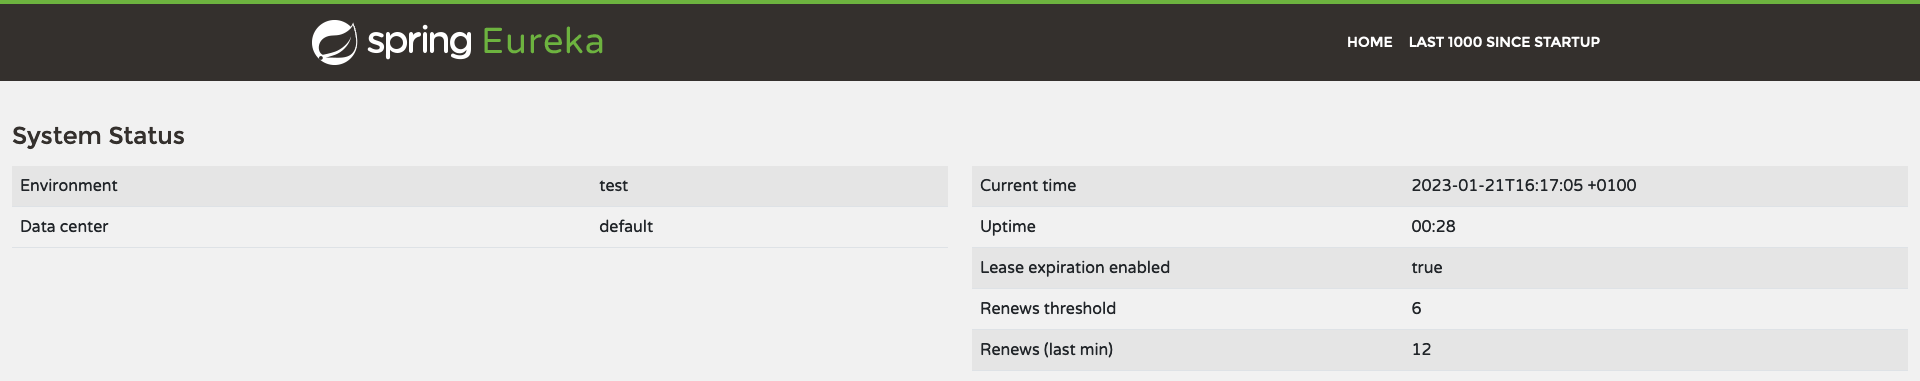
\includegraphics[scale=0.20]{capitoli/immagini/13_general_info.png}
    \caption{Informazioni generali sul servizio Eureka}
    \label{fig:General_info}
\end{figure}

Nella stessa pagina possibile non solo verificare lo stato del discovery service, ma anche i servizi registrati, il loro stato e il loro indirizzo di registrazione locale in tempo reale.

\begin{figure}[h]
    \centering
    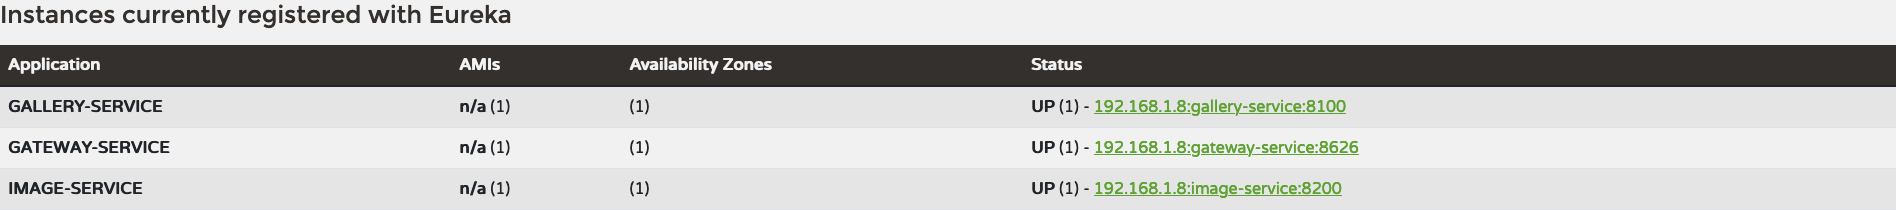
\includegraphics[scale=0.20]{capitoli/immagini/14_subscribe_services.png}
    \caption{Informazioni sui microservizi sottoscritti ad Eureka}
    \label{fig:Subscribe_Services}
\end{figure}

\subsection{Gateway Service}
Spring Cloud Gateway \cite{gateway} ha l'obiettivo di fornire un meccanismo di instradamento ai servizi che permetta di mantenere aspetti come la sicurezza e il monitoraggio delle risorse.

\begin{figure}[h]
    \centering
    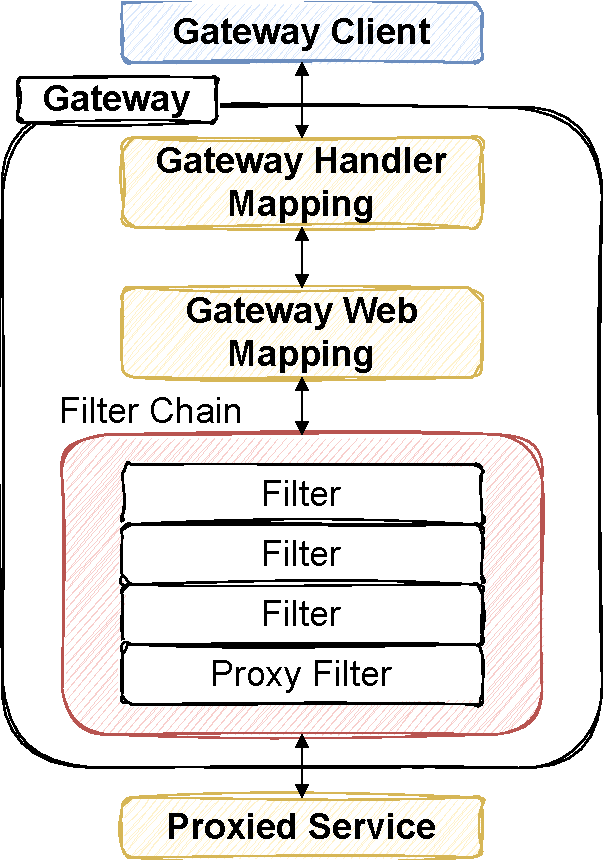
\includegraphics[scale=0.65]{capitoli/immagini/15_gateway_work.pdf}
    \caption{Funzionamento di Spring Cloud Gateway}
    \label{fig:gateway_work}
\end{figure}

Quando il servizio riceve una richiesta da un client, il componente Gateway Handler Mapping si occupa di riconoscere se il percorso inserito è corretto, in caso affermativo invia la richiesta al Gateway Web Handler che gestisce la richiesta, quest'ultima passa attraverso ad una serie di filtri che implementano logica di sicurezza, ed infine si collega al servizio richiesto dal client.

Durante la configurazione di tale servizio è necessario specificare i vari percorsi dei servizi. Nel nostro caso dobbiamo specificare due servizi, Image Service e Gallery Service, in questo modo il gateway sarà instruito su come instradare il traffico dei dati. Nel file application.properties specifichiamo tre attributi principali:

\begin{lstlisting}[caption=Application.properties del Gateway]
spring.cloud.gateway.routes[0].id=gallery
spring.cloud.gateway.routes[0].uri=lb://GALLERY-SERVICE
spring.cloud.gateway.routes[0].predicates[0]=Path=/gallery/**

spring.cloud.gateway.routes[1].id=image
spring.cloud.gateway.routes[1].uri=lb://IMAGE-SERVICE
spring.cloud.gateway.routes[1].predicates[0]=Path=/image/**
\end{lstlisting}

Possiamo notare che gli URI presenti nella configurazione coincidono con i nomi dei servizi che sono registrati sul server eureka \ref{fig:General_info}, questo perché il Gateway andrà a ricercare questi servizi proprio nel server di Eureka, nel caso i nomi non coincida quando si andrà a richiedere al Gateway di instradare del traffico verso un servizio quest'ultimo restituirà una pagina di errore.

Sempre nell'URI è possibile osservare che prima di ogni nome di servizio compare "lb", il gateway oltre all'instradamento del traffico si occupa anche di applicare una politica di load balancer, in modo da poter gestire il carico di lavoro in entrata e in uscita.


\begin{comment}
\subsection{Image Service - Logica di Business}

\begin{lstlisting}[language=Java]
@RestController
@RequestMapping(path = "/image")
public class HomeController {
    @Autowired
    private Environment env;
    @RequestMapping
    public String Home() {
        return "Hello from Image Service runnig at port: " + env.getProperty("local.server.port");
    }
    @RequestMapping(path = "/all")
    public List<Image> getImages() {
        return Arrays.asList(
                new Image(1, 
                        "Treehouse of Horror V", 
                        "https://www.imdb.com/title/tt0096697/mediaviewer/rm3842005760"),
                new Image(2, 
                        "The Town", 
                        "https://www.imdb.com/title/tt0096697/mediaviewer/rm3698134272"),
                new Image(3, 
                        "The Last Traction Hero", 
                        "https://www.imdb.com/title/tt0096697/mediaviewer/rm1445594112"));
    }
}
\end{lstlisting}

\subsection{Gallery Service - Logica di Business}

\begin{lstlisting}[language=Java]

@RestController
@RequestMapping(path = "/gallery")
public class HomeController {

    @Autowired
    private RestTemplate restTemplate;

    @Autowired
    private Environment env;

    @RequestMapping
    public String Home() {
        return "Hello from Gallery Service runnig at port: " + env.getProperty("local.server.port");
    }
    @RequestMapping(path = "/{id}")
    public Gallery getGallery(@PathVariable final int id){
        Gallery gallery = new Gallery();
        gallery.setId(id);

        List<Object> images = restTemplate.getForObject("http://image-service/image/all", List.class);
        gallery.setImages(images);

        return gallery;
    }
    @RequestMapping(path = "/admin")
    public String homeAdmin(){
        return "this is the admin area of Gallery Service running at port: " + env.getProperty("local.server.port");
    }
}

\end{lstlisting}
\end{comment}

\subsection{Avvio dei servizi}
L'ordine di deploy dei servizi è importante, il discovery service deve essere il primo servizio ad essere disponibile questo perché i vari servizi appena avviati invieranno una richiesta di registrazione e se Eureka è offline i servizi si arresteranno con un errore. L'ordine utilizzato per l'avvio dell'applicativo è il seguente:

\begin{enumerate}
    \item Eureka Server Service;
    \item Image Service;
    \item Gallery Service;
    \item Gateway Service;
\end{enumerate}

L'ordine di avvio del gateway non è importante, il servizio in questione effettuerà periodicamente una chiamata ad Eureka per verificare la presenza di nuovi servizi, se presenti verificherà il nome di quest'ultimi con i nomi specificati nel proprio file di configurazione.

\section{Aggiunta di un nuovo servizio}
Abbiamo detto più volte che grazie all'approccio ai microservizi andiamo a creare un software modulare con i servizi che sono indipendenti gli uni dagli altri, questo ci dice che è anche possibile implementare nuove tecnologie molto più facilmente.

\subsection{World Service}
World è il risultato del lavoro svolto durante l'attività di tirocinio presso Kineton. Sviluppato con Spring Boot, tale servizio si basa sul database world, una banca dati messa a disposizione gratuitamente dal sito di MySQL. Per prima cosa andiamo a modificare il diagramma dell'architettura visto precedentemente per implementare questo nuovo servizio:

\begin{figure}[h]
    \centering
    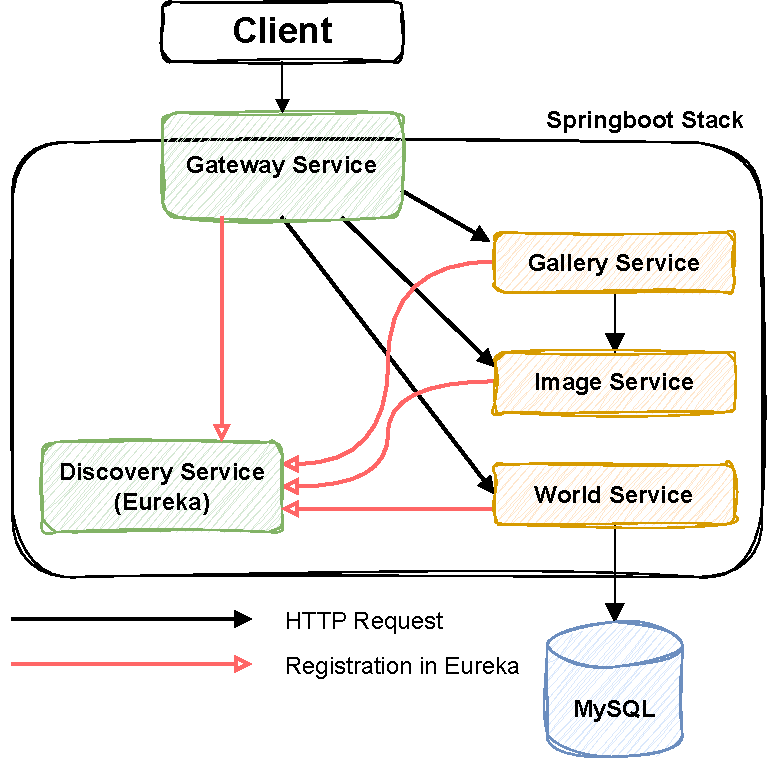
\includegraphics[scale=0.65]{capitoli/immagini/16_architettura_world.pdf}
    \caption{Architettura modificata con l'aggiunta di World Service}
    \label{fig:new_architecture}
\end{figure}

Oltre ad aver inserito il servizio che si occupa di esporre le API facciamo anche affidamento su un database che contiene i nostri dati.

\paragraph{Diagramma Entità Relazione di World}
Il diagramma ER del database World è formato da tre tabelle. Le due tabelle countrylanguage e city sono in relazione con la tabella country tramite una relazione uno a molti.
Nella tabella countrylanguage, l'attributo Language è una chiave primaria per la tabella e l'attributo countryCode è dichiarata come chiave primaria e come chiave esterna che fa riferimento al'attributo Code di country. Anche nella tabella city l'attributo CountryCode è una chiave esterna, che fa riferimento all'attributo Code di country. Infine in country la chiave primaria è Code.

\begin{figure}[h]
    \centering
    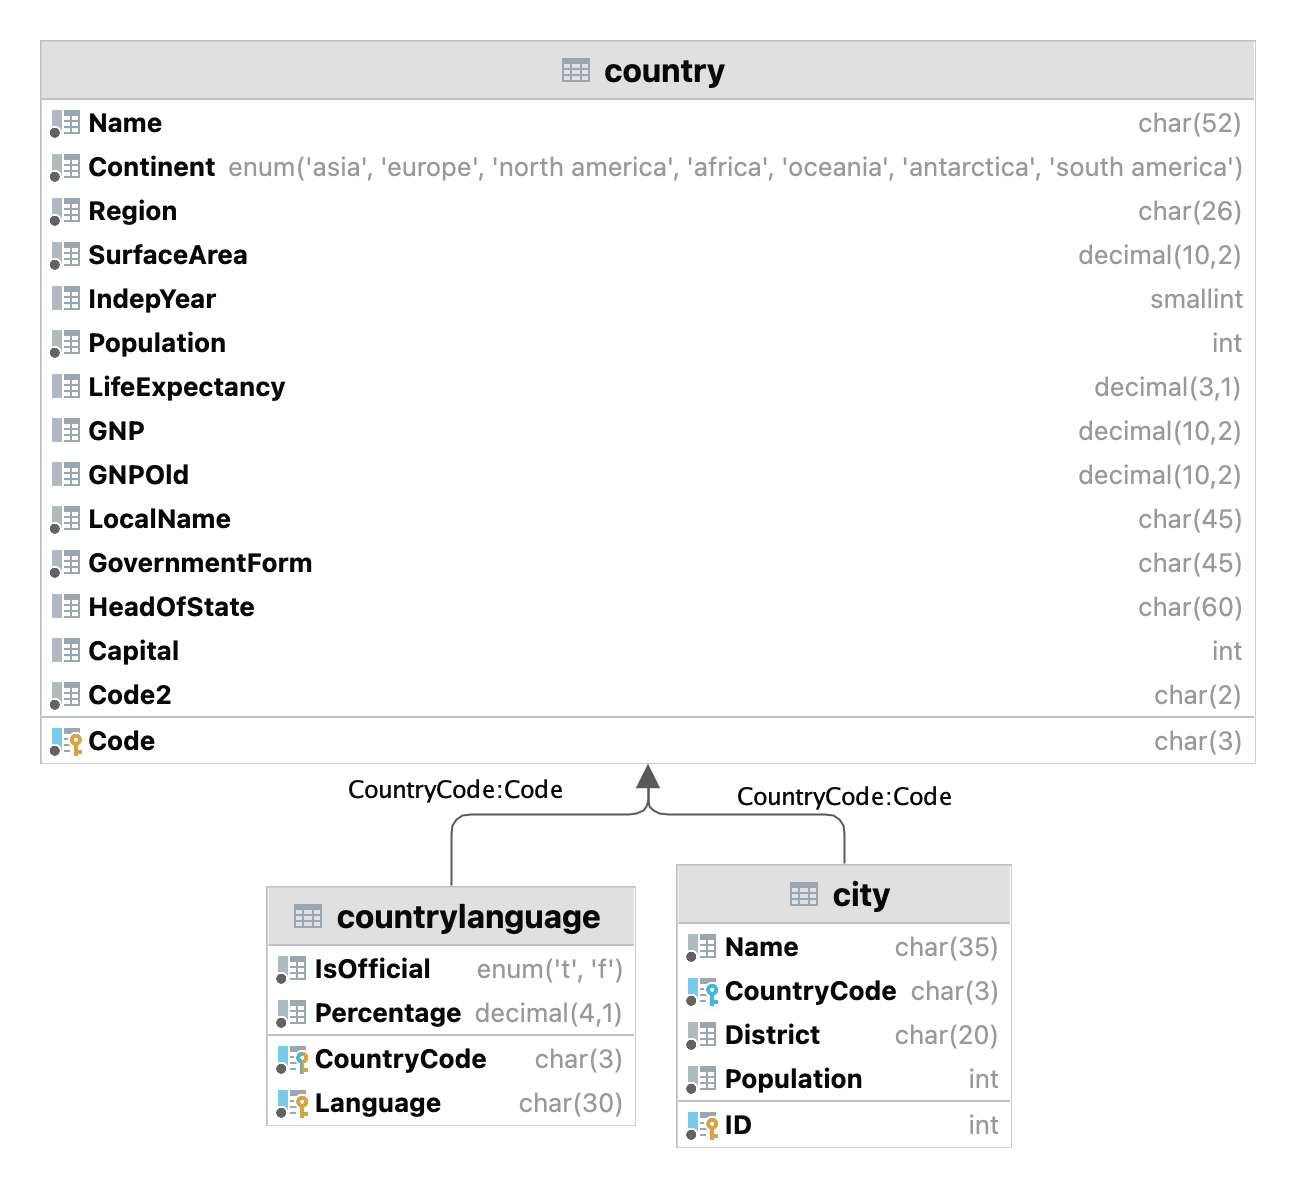
\includegraphics[scale=0.25]{capitoli/immagini/17_world_database.png}
    \caption{Diagramma del Database World}
    \label{fig:database}
\end{figure}

\subsection{Modifiche}
Una volta importato il progetto i cambiamenti da effettuare lato codice sono semplici. Prima di tutto dobbiamo dichiarare una nuova dipendenza. L'applicazione era stata creata per esporre delle API, non era previsto il suo ingresso in un'applicazione basata sui microservizi, quindi nel pom andremmo ad aggiungere la dipendenza per poter far si che il servizio possa essere scoperto da Eureka:

\begin{lstlisting}[language=xml, caption= Dipendenza di Eureka Client]
<dependency>
    <groupId>org.springframework.cloud</groupId>
    <artifactId>spring-cloud-starter-netflix-eureka-client</artifactId>
    <version>3.1.4</version>
</dependency>
\end{lstlisting}

Nel file di configurazione dobbiamo dare un nome al nostro servizio per poter essere registrato, una porta diversa dalla configurazione di base di Spring Boot (la porta 8080) e infine dobbiamo specificare l'URL del servizio di discovery Eureka:
\begin{lstlisting}[caption = Configurazione per Eureka]
#Eureka Client
spring.application.name=WORLD-SERVICE

server.port=8000
eureka.client.service-url.default-zone=http://localhost:8761/eureka
\end{lstlisting}

L'ultima modifica che dobbiamo effettuare è al file di configurazione del servizio che offre il Gateway. Questo perché, come visto in precedenza il gateway deve poter riconoscere l'instradamento dei servizi, quindi non ci resta che aggiungere il percorso per il nostro nuovo servizio:

\begin{lstlisting}[caption= Configurazione per il Gateway]
spring.cloud.gateway.routes[2].id=world
spring.cloud.gateway.routes[2].uri=lb://WORLD-SERVICE
spring.cloud.gateway.routes[2].predicates[0]=Path=/api/**
\end{lstlisting}

Una volta effettuato il deploy di tutti i servizi, possiamo notare sulla dashboard di Eureka che il nostro servizio è attivo ed è stato registrato:

\begin{figure}[h]
    \centering
    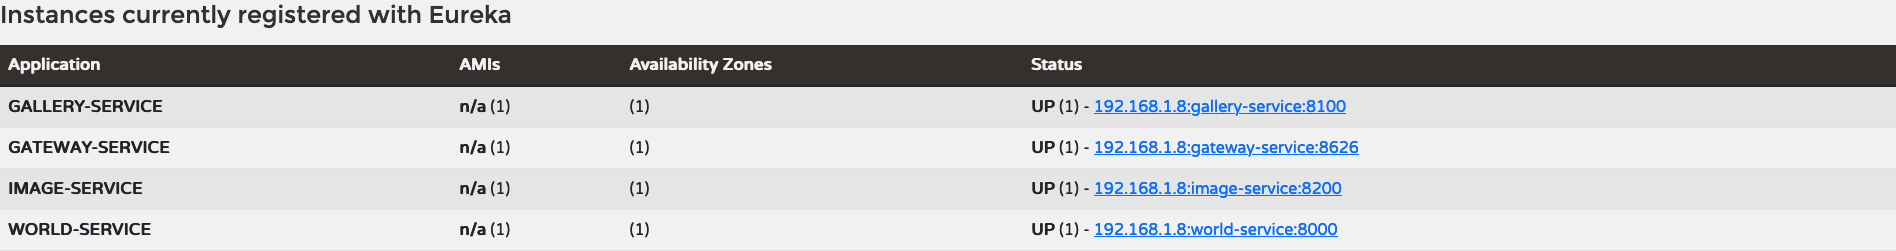
\includegraphics[scale = 0.20]{capitoli/immagini/18_world_eureka.png}
    \caption{World Service è registrato su Eureka}
    \label{fig:world_eureka}
\end{figure}
\chapter{Conclusioni}
Lo scopo di questo lavoro era quello di presentare il modello architetturale basato sui microservizi. L'avanzamento delle tecnologie ha portato ad una crescente richiesta di software sempre più impegnativi, l'approccio di sviluppo col modello monolitico inizia a non essere più la scelta più ideale.

Abbiamo discusso di alcune delle tecnologie che implementato concetti teorici di inizi anni 2000 e abbiamo presentato un lavoro che basato sull'approccio ai microservizi ha reso evidente i vantaggi offerti da questa architettura. Le tecnologie che negli anni si sono perfezionate hanno migliorato sempre di più l'architettura ai microservizi, ciò che prima poteva creare dei problemi oggi è stato risolto tramite diverse tecnologie.

Buffo, per la creazione di un applicativo a microservizi abbiamo dovuto far affidamento su diverse tecnologie che offrissero diversi servizi e a sua volta ogni strumento utilizzato e stato creato facendo affidamento ad altri servizi. Questa ridondanza è ciò che rende questo approccio così versatile è potete, non importa come un servizio sia stato scritto o implementato.

Con il sempre più crescente interesso verso il cloud computing, le applicazioni e i software stanno cambiando drasticamente.


\backmatter
\phantomsection
\chapter{Ringraziamenti}
Siamo giunti alla fine di un lungo percorso. Prima di tutto vorrei ringraziare tutte le persone che hanno letto e sono riusciti ad arrivare fino a questo punto.

Ringrazio la professoressa \textbf{Rita Francese} che mi ha dato l'opportunità di svolgere il mio lavoro di tirocinio esternamente presso Kineton e che col suo corso di Tecnologie e Software per il web oggi sto entrando nel mondo dello sviluppo di applicazioni web.

Tutti le persone e ormai colleghi di Kineton che mi hanno seguito nei mesi precedenti nello studio di queste tecnologie, in particolare il mio tutor \textbf{Paolo Nappi} e \textbf{Valentino Vivone}.

I miei amici e colleghi universitari, in particolare \textbf{Michele Brignola}, \textbf{Giuseppe Arienzo}, \textbf{Alessandro D'Onofrio}, \textbf{Mattia Mascolo} e \textbf{Andrea Raiola} che sono riusciti a sopportare il mio caratteraccio durante questi anni universitari e che hanno ritardato il conseguimento di questo titolo.

Mio zio \textbf{Rosario} che mi ha sempre motivato e incoraggiato e il mio cane \textbf{Ciccia} che mi ha fatto compagnia durante i pisolini pomeridiani di ritorno dall'università

Per finire vorrei ringraziare la persona che mi sta supportando da circa 25 anni, mia \textbf{Mamma}, nei momenti buoi della carriera universitaria c'è sempre stata e ha sempre appoggiato il mio percorso. Grazie.

\begin{figure}
    \centering
    
\includegraphics[scale=0.10]{capitoli/immagini/thankyou.png}
\end{figure}


\printbibliography
\end{document}